%!TEX encoding = UTF-8 Unicode

% Load Thesis Class
\documentclass{DEIThesis}

\title{Development of a virtual reality application for the training of cardiac surgeons}

\author{Boscolo Cegion Nicola}
\studentId{2074285}

% Advisor
\advisor{Prof. Savino Sandro}
\graphicspath{ {./res/} }

\university{University of Padua}
\mastername{Computer Engineering}
\academicYear{2023/2024}

\begin{filecontents*}[overwrite]{\jobname.xmpdata}
    \Title{Development of a virtual reality application for the training of cardiac surgeons}
    \Author{Boscolo Cegion Nicola}
    \Language{en-EN}
    \Keywords{Computer Engineering\sep LaTeX}
\end{filecontents*}

% Document

\begin{document}
    % The front matter (Cover, ToC, Abstract, etc...)
    \frontmatter

    % The main content
    \mainmatter
    
    %!TEX root = ../main.tex

\chapter{Introduction}
\label{chp:intro}

\section{Case introduction}

At the university hospital of Padua, 
there is a very important cardiac surgery center where various heart interventions are performed on many people,
the need to teach and visualize the case of operation is very important. \\
Thanks to MRI, surgeons can see not only pictures of the heart, but also can even make 3D models.
Each 3D model can show every detail of the patient's heart, this can make surgeons able to analyze and show where and how to resolve the problem.

\subsection{Virtual reality head mounted displays}

\paragraph{The equipment:}
The equipment: The university of Padua has some Meta quest 2\footnote{All rights to meta reserved} [fig:\ref{fig:metaQuest2}] a \ac{HMD} for \ac{VR}.\\ 
The Meta Quest 2 is a standalone \ac{HMD}, this means that it doesn’t need other peripherals like an external console or \ac{PC} for working.\\
For user interaction, the Meta Quest 2 uses two wireless controllers, but it also has the possibility to use hand-tracking, to let the user navigate the interfaces by using his/her own hands.
The tracking of the user in the real-world environment is achieved using 4 infrared cameras and other sensors like multi axes gyroscopes and accelerometers.\\
They use a custom version of the Android \ac{OS}, this can give a certain degree of liberty in creating APPs for the device.

\begin{figure}[h]
  \centering
  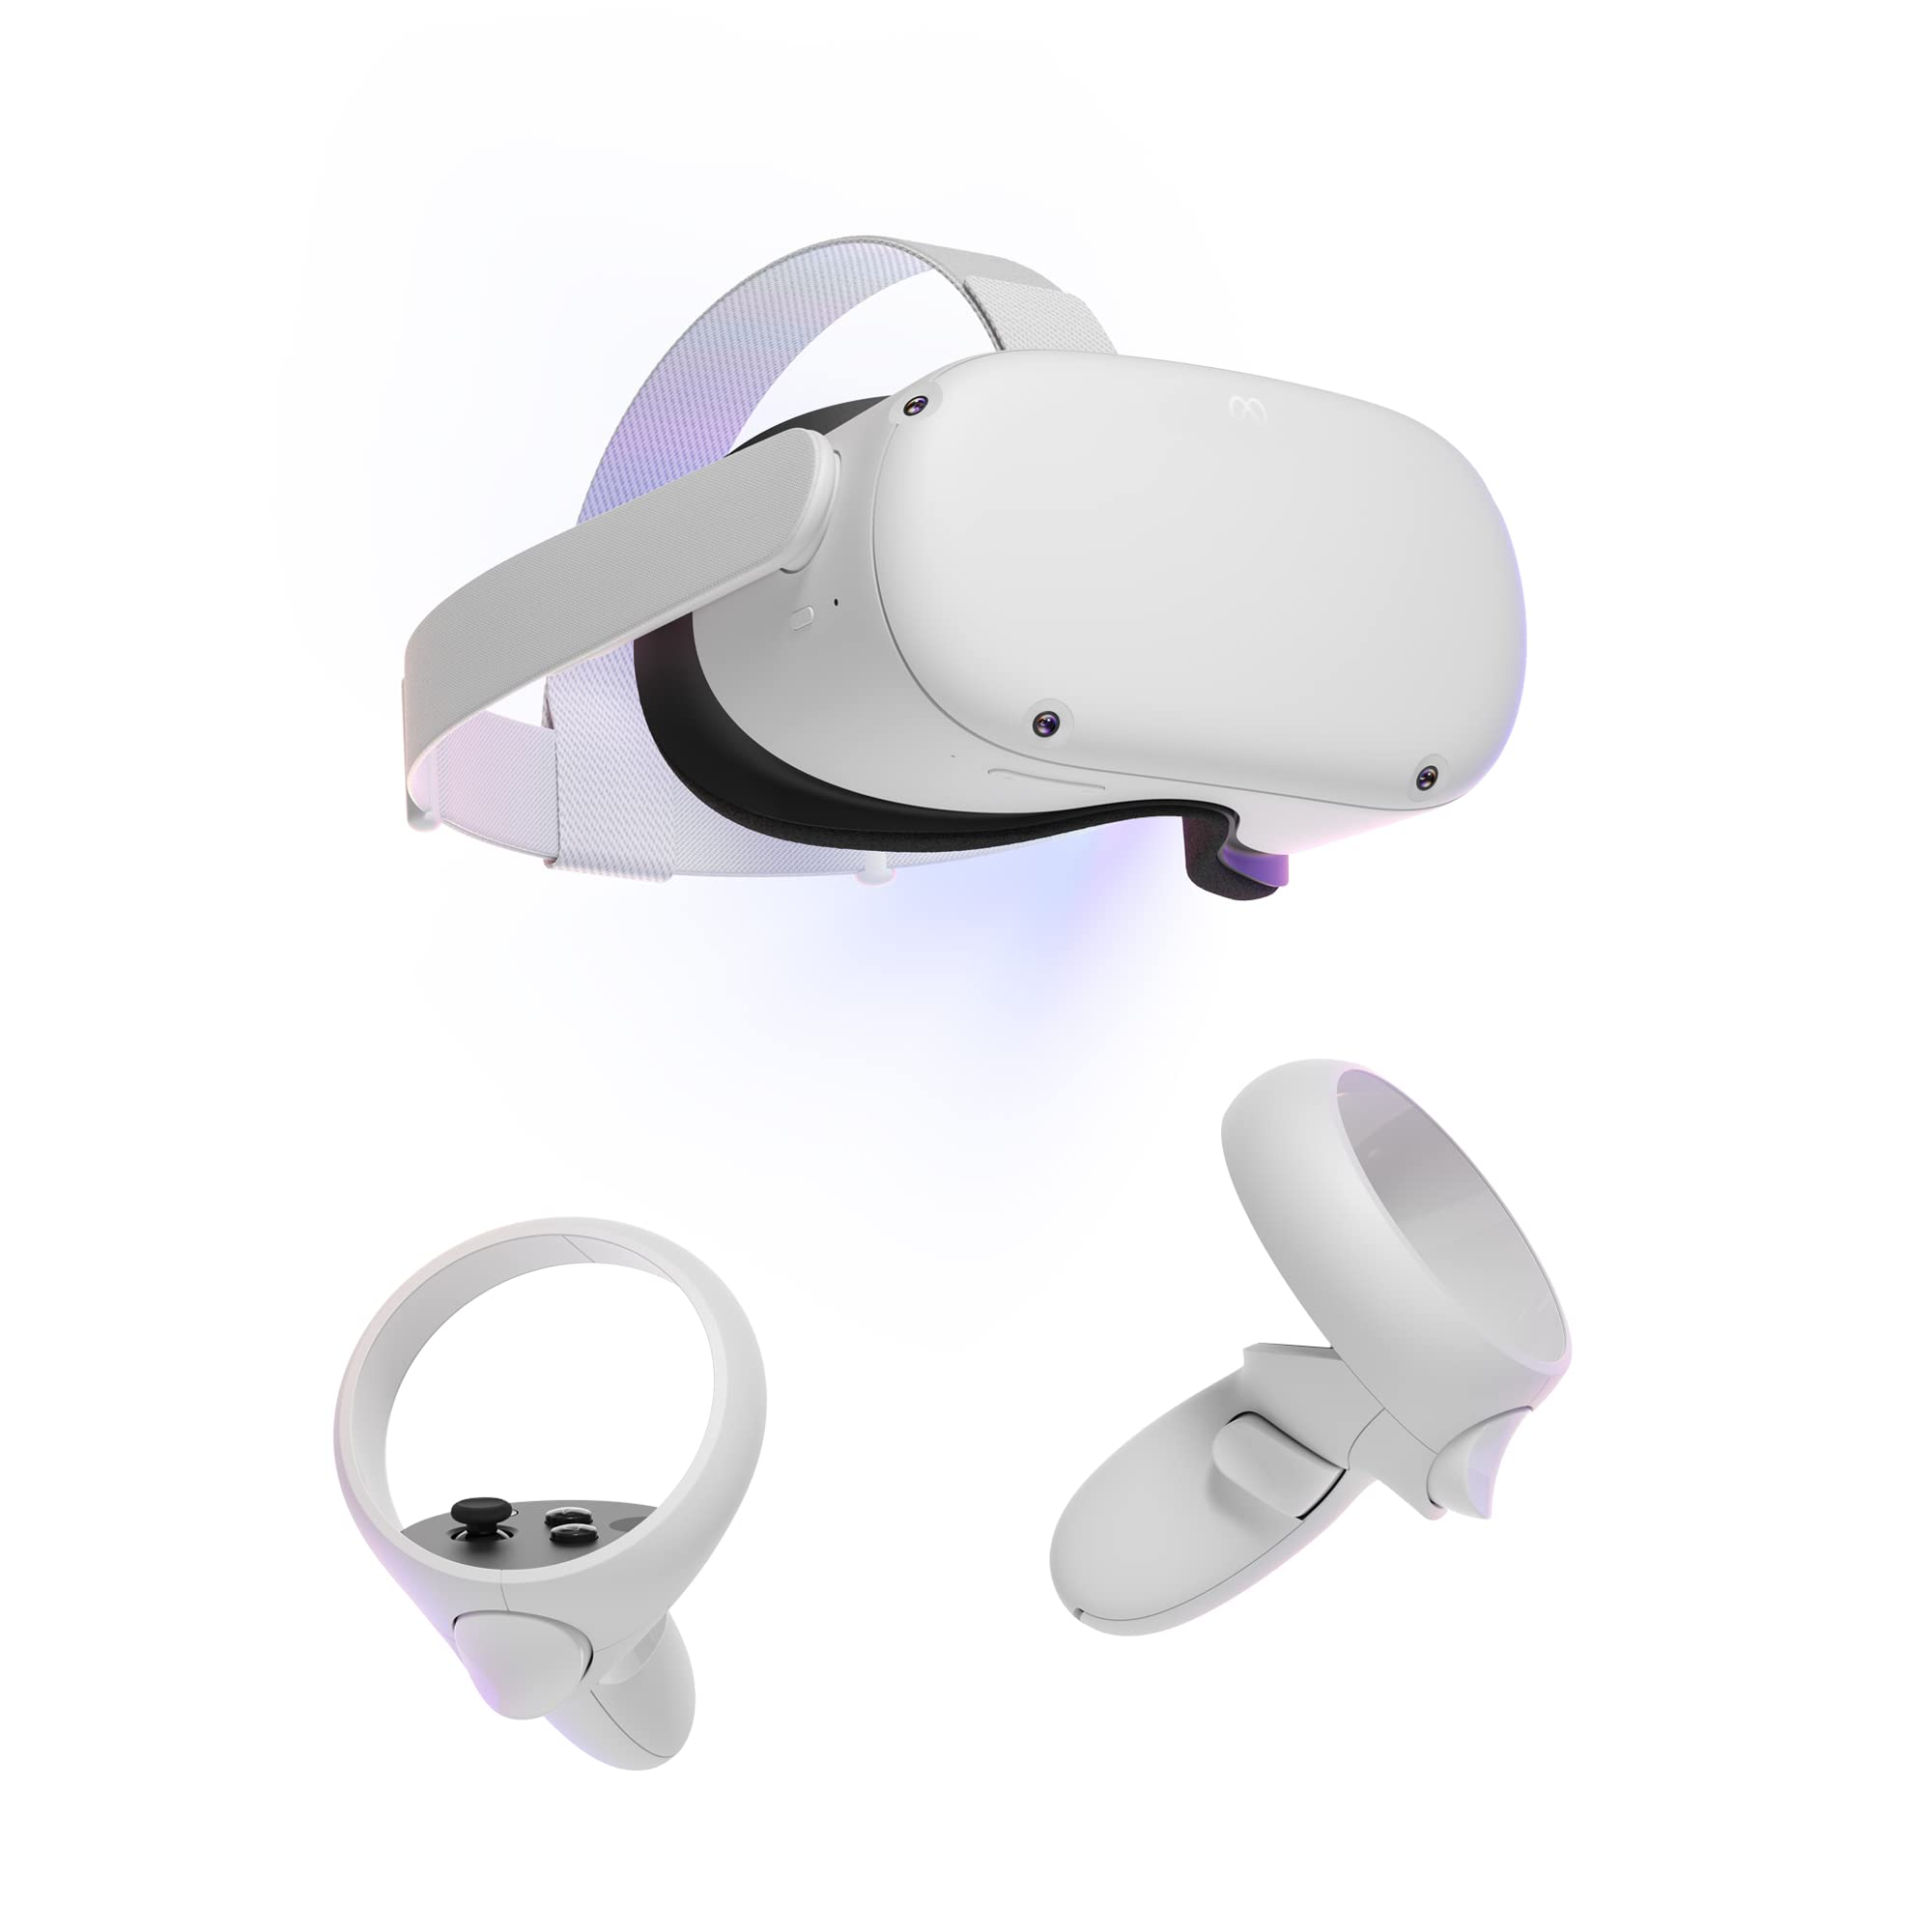
\includegraphics[width=0.5\textwidth]{metaQuest2.jpg}
  \caption{Meta quest 2}
  \label{fig:metaQuest2}
\end{figure}

\paragraph{Use cases of VR:}
Principally the surgeons are using VR equipment for training and showing critical health conditions of different patients' hearts.
They are using an APP called Shapes XR, this APP has a web interface for uploading 3D models and then showing them on the \ac{HMD}.
The app has a multiplayer functionality so that multiple people can look at the 3D models in the environment, even if the developers recommend at max 8 people, they tested with 14 users connected and there weren't any problems.

\subsection{APP problems}

\paragraph{How Shapes XR works:}
Shapes XR lets you create rooms, accessible via a code, where multiple people can create 3D models with basic tools like 3D brushes and standard shapes like cubes, pyramids and so on.
It also lets you upload a 3D model file on their own website, so that in the home you can download it and start to work on it.
It lets you also create your own avatar.
This is the main feature that the surgeons are using for show the 3D Models

\paragraph{The Problems:}
Unfortunately Shapes XR is principally used for 3D modeling, so the app has a lot of features like changing the scale of the world or brushes for modeling the objects that aren't useful for the surgeons,
and quite distracting because for a lot of people it is the first time using a \ac{HMD}.\\
The user experience is extremely important in \ac{VR} because it is difficult to tutoring the user while using the \ac{HMD}.
Then Shapes XR positions the user in an empty 3D plane with little to none point of reference so If a user accidentally uses the teleport function, they may find themselves somewhere far away from the scene they are supposed to be watching.

\paragraph{Feedbacks from surgeons and nurses:}

There was a lesson on 12/12/2023 with the integration of the Quest 2 and Shapes XR. First it was pretty chaotic, a lot of people did not even know how to use the controllers,
 and they had problems even putting in the code for entering the session. Unfortunately we did not have time to make a nice lesson for teaching how to use the HMD,
  the tutorial made by Meta approximates takes 15 min to complete, even more if the user wants to try the mini-games, so we did not have the time to show it. The main critical points were: 

\begin{itemize}
  \item Inadequate tutoring for teaching how to use the \ac{HMD}
  \item Difficulty for accessing the multiplayer room
  \item Difficulty at moving in the room
  \item Some people avatar were blocking the visual of some people
\end{itemize}
\noindent
How we can see a new app for this use case could be useful, and this is the main reason why this project exists. 
    %!TEX root = ../main.tex

\chapter{Starting situation}
\label{chp:starting situation}

\begin{figure}[ht]
    \centering
    
\includegraphics[width=0.5\textwidth]{res/ltunipd}
    \caption{Example of image}
\end{figure}
    %!TEX root = ../main.tex

\chapter{Preliminary project}

\section{The game engine}

\paragraph{What to choose?:} 
There are three main way to develop on the Meta Quest 2:

\begin{itemize}
  \item \textbf{Native:} By using native \ac{API} that Meta provides for the \ac{HMD}.
  \item \textbf{Unity:} Is a famous game engine principally used for lightweight video games, It is pretty functional and easy to use, its programming language is C\#.
  \item \textbf{Unreal Engine:} Is a famous game engine used for big games, its performance is the best in the market, it uses C++ and a graphical programming language called Blueprint.
\end{itemize}
\noindent
As we said in the non-functional requirements we will use a game engine, I have opted for \ac{UE} because of its performance, the 3D models are pretty complex (\textasciitilde10MByte in size),
so we need good performance.
It has a lot of tools for multiplayer and a nice documentation other than a big community of developers.

\section{Unreal Engine}
\noindent
Made by Epic Games, the project was born for the video game Unreal, now is one of the best engine that power a lot of important video games and 3D animation.
For this project it will be used the 5.2.1 version for the best compatibility with the \ac{HMD}, still is not a very old version, the last one is 5.3. 

\paragraph{The fundamentals:}
\ac{UE} has a 3D preview mode that let the user set the various 3D objects in the scene. 
In unreal a scene is called "Level", each element in a level is called "Actor", Actors are made by multiple components.\\
Each element of unreal can be build with a propriety system called Blueprint, a visual programming interface, or via C++, or by combine them.
Principally Blueprint can make the developing of the project faster and easier at the cost of performance, C++ perform better, and it has a bigger range of tools.
So It is important to combine both languages for having the best performance and flexibility in the project.\\
Like a lot of game engines, \ac{UE} tries to render as much frame as much as possible, each cycle of rendering is called tick.\\
Its important that long actions must be asynchronous respect the game ticks, and if something must be runner in the so-called "game thread", it must be as fast as possible so that the frame rate does not drop to a certain level.

\paragraph{Events:}
Events are what start the execution of code inside a Blueprint. Each blueprint have its own standard event, they depend on the object, the basic ones are:
\begin{itemize}
  \item \textbf{Begin Play:} runs one time when the actor is spawned (this is not a constructor).
  \item \textbf{On tick:} runs on every game tick.
\end{itemize}
\noindent
But we can also create custom event with Blueprint or C++, they can be triggered whenever we want, they can also be replicated in clients in multiplayer sessions. 
Like functions, events can have inputs but not outputs.

\paragraph*{Multiplayer:}
\ac{UE} just support a client-server configuration for manage multiplayer session, it has two main implementation: Stand-Alone server and listening server.\\
Stand-Alone server consist in having a server that emulates the gaming session, it requires a server powerful enough to run the basic function of the game event if it does not need to render it.\\
Listening Server does not need a Stand-Alone server, simply one device acts not only as a client but also as a server. Normally client-server is the best in performance and latency, but because this software is simple, the listening server is the right implementation.

\section{Network Infrastructure}
\noindent
The Network Infrastructure [fig:\ref{fig:NetworkSchema}] it is simple, a server will be hosted in the IT department of the hospital that will host the \ac{REST} server for managing 3D Models and multiplayer sessions,
and in the same server will host via NODEjs the Web Portal for managing the 3DModels.
The multiplayer itself will be manage by the host \ac{HMD}

\begin{figure}[h]
  \centering
  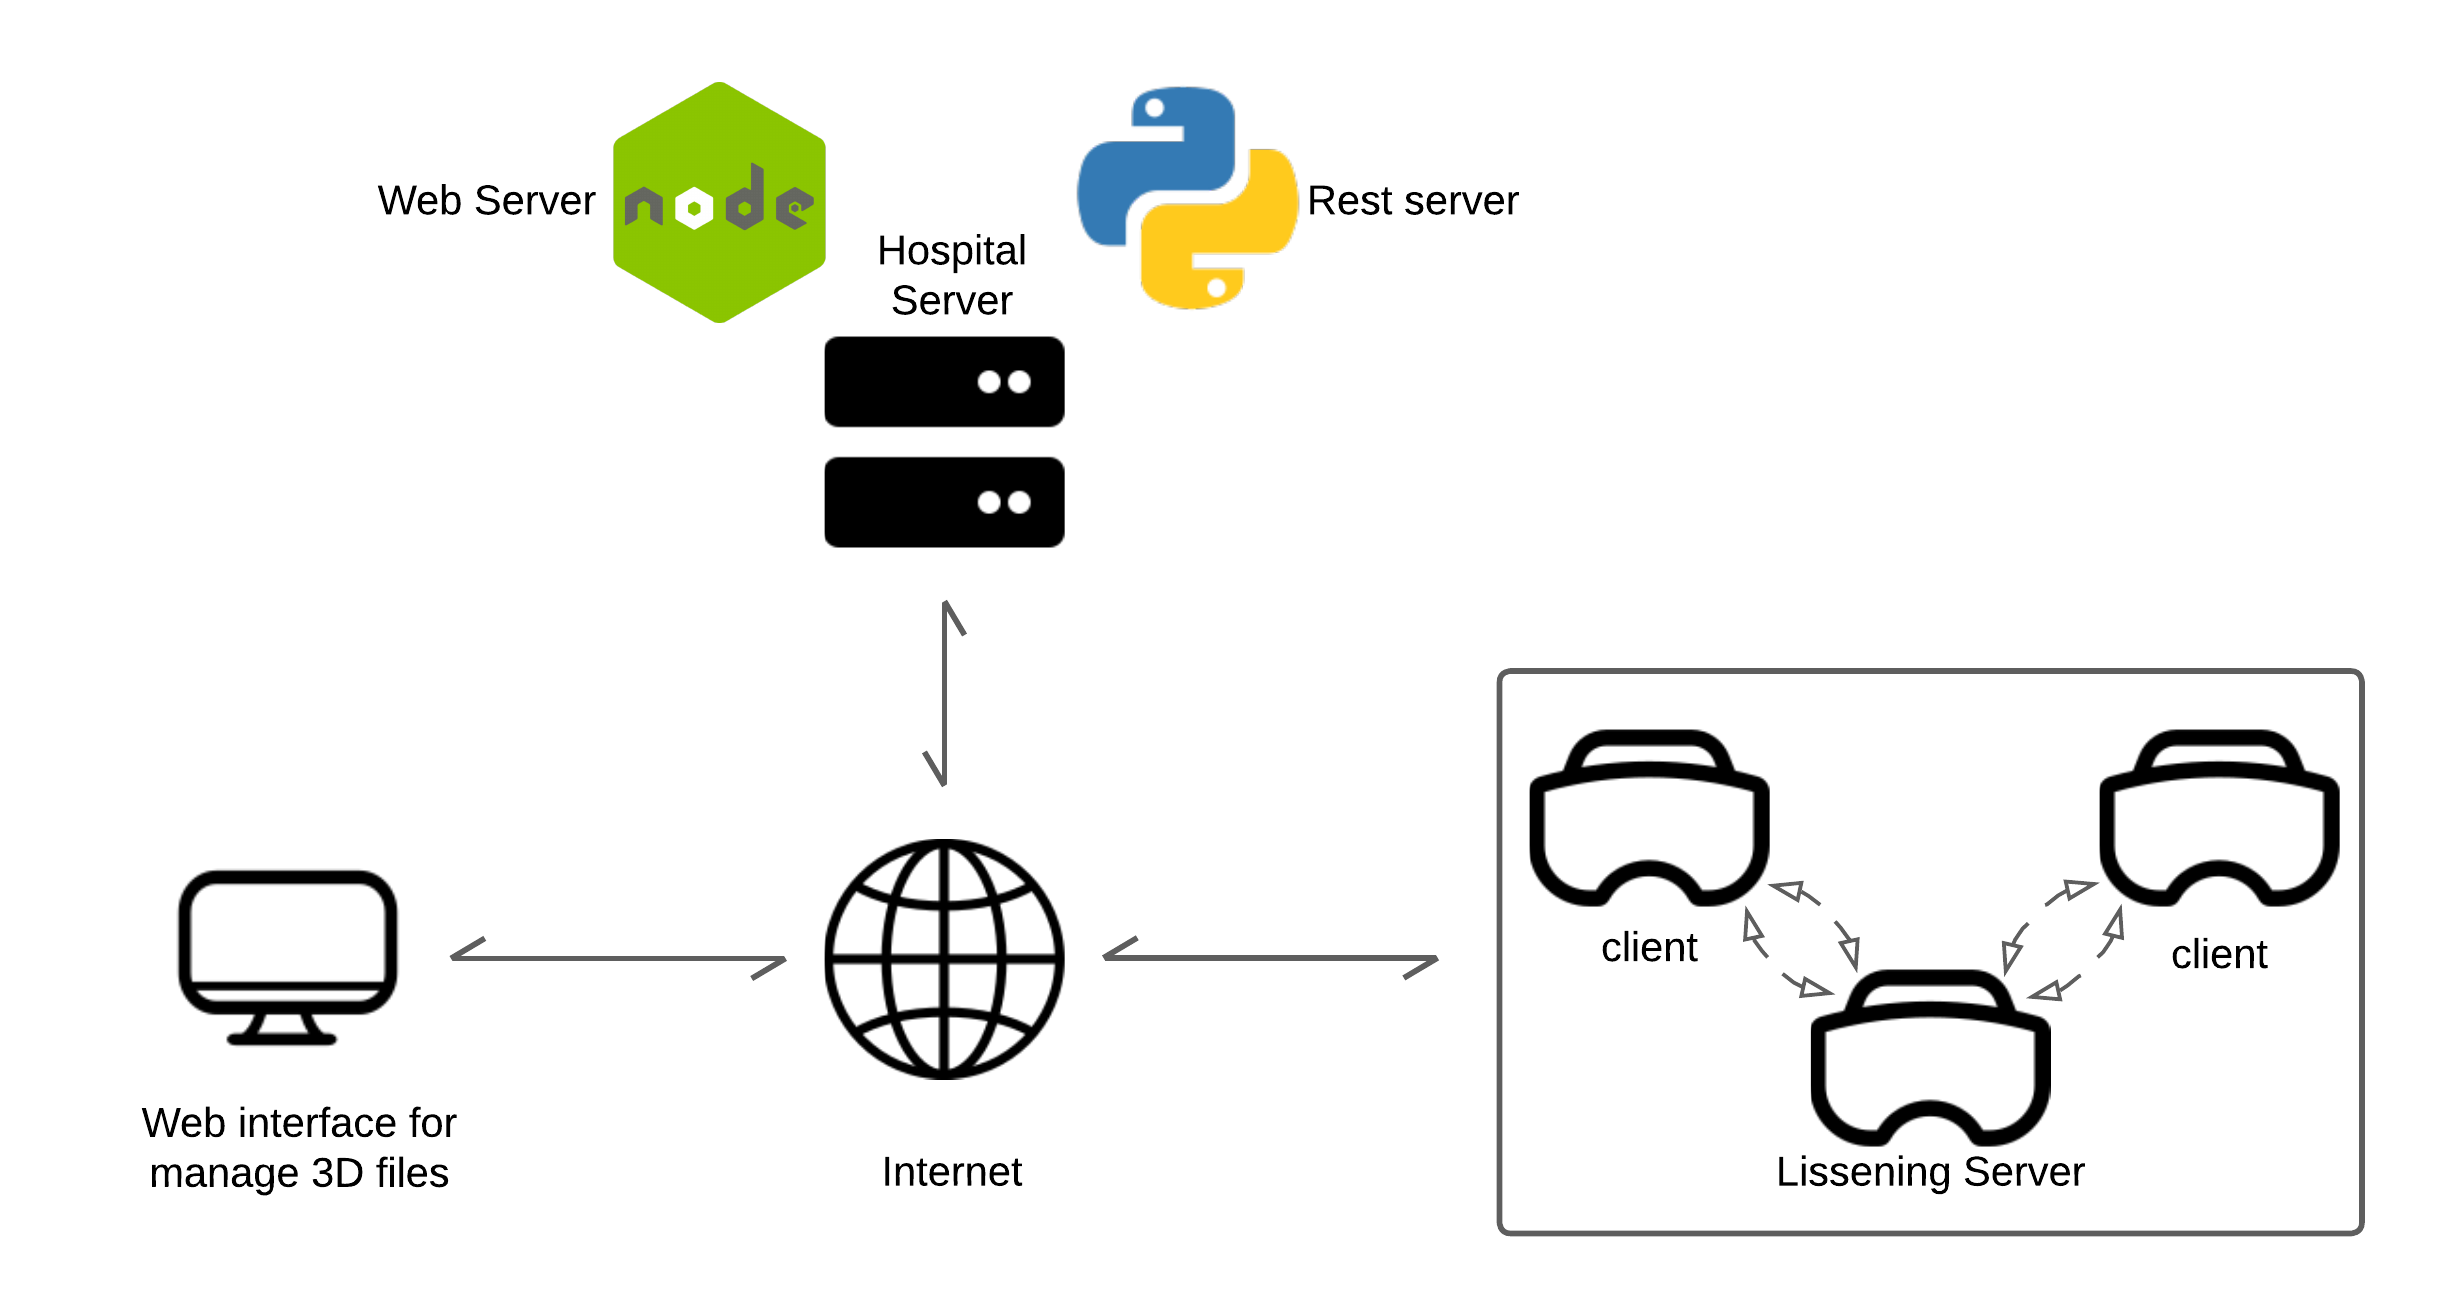
\includegraphics[width=\textwidth]{networkSchema.png}
  \caption{Network Schema}
  \label{fig:NetworkSchema}
\end{figure}


\paragraph{The backend:}
The backend is a simple Python program that it functions as a \ac{REST} server, were each 3D model is a resource.
It also manages the multiplayer session by creating the session code, and save the \ac{IP} address of the listening server.
The library used is called Flask\footnote{\url{https://flask.palletsprojects.com/en/3.0.x/}}, it simply let you run a function respect to a \ac{HTTP} response received.

\paragraph{The WebUI}
The WebUI is made with reactJS, a popular framework for website, the main reason of this choice is for faster development because its community is massive, in fact will be using a UI library called MUI\footnote{\url{https://mui.com/}}
and a 3D library for rendering 3D models called React Three Fiber\footnote{\url{https://r3f.docs.pmnd.rs/getting-started/introduction}}.\\
The main functionality of the WebUI will be:
\begin{itemize}
  \item previewing 3D models
  \item upload 3D models
  \item delete 3D models
\end{itemize}



    %!TEX root = ../main.tex

\chapter{Analysis of the requirements}
\label{chp:requirements}

\begin{algorithm}[ht]
    \caption{An algorithm with caption}\label{alg:two}
    \begin{algorithmic}
        \REQUIRE $n \geq 0$
        \ENSURE $y = x^n$
        
        \STATE $y \gets 1$
        \STATE $X \gets x$
        \STATE $N \gets n$
        
        \WHILE{$N \neq 0$}
            \IF{$N$ is even}
              \STATE $X \gets X \times X$
              \STATE $N \gets \frac{N}{2} $  \COMMENT{This is a comment}
            \ELSIF{$N$ is odd}
              \STATE $y \gets y \times X$
              \STATE $N \gets N - 1$
            \ENDIF
        \ENDWHILE
    \end{algorithmic}
\end{algorithm}

\begin{equation}
e^{j\pi} + 1 = 0
\end{equation}
    %!TEX root = ../main.tex

\chapter{The project}
\label{chp:project}

\section{A section}

\tikzset{vertex style/.style={
    draw=#1,
    thick,
    fill=#1!70,
    text=white,
    ellipse,
    minimum width=2cm,
    minimum height=0.75cm,
    font=\small,
    outer sep=3pt,
  },
  text style/.style={
    sloped,
    text=black,
    font=\footnotesize,
    above
  }
}

\begin{figure}[ht]
    \centering
    \begin{tikzpicture}[node distance=2.75cm,>={Stealth[]}]
        \node[vertex style=cyan] (Rk) {Righteous Kill};
        \node[vertex style=orange, above of=Rk,xshift=2em] (BD) {Bryan Dennehy}
        edge [<-,cyan!60!blue] node[text style,above]{starring} (Rk);
    \end{tikzpicture}
    
    \caption{Image created with TikZ} \label{fig:T1}
\end{figure}

\paragraph{}
Lorem ipsum dolor sit amet, consectetur adipiscing elit, sed do eiusmod tempor incididunt ut labore et dolore magna aliqua. Ut enim ad minim veniam, quis nostrud exercitation ullamco laboris nisi ut aliquip ex ea commodo consequat. Duis aute irure dolor in reprehenderit in voluptate velit esse cillum dolore eu fugiat nulla pariatur. Excepteur sint occaecat cupidatat non proident, sunt in culpa qui officia deserunt mollit anim id est laborum.

\begin{lstlisting}[language=Python, caption=Code snippet example]
import numpy as np
    
def incmatrix(genl1,genl2):
    m = len(genl1)
    n = len(genl2)
    M = None #to become the incidence matrix
    VT = np.zeros((n*m,1), int)  #dummy variable

    test = "String"
    
    #compute the bitwise xor matrix
    M1 = bitxormatrix(genl1)
    M2 = np.triu(bitxormatrix(genl2),1) 

    for i in range(m-1):
        for j in range(i+1, m):
            [r,c] = np.where(M2 == M1[i,j])
            for k in range(len(r)):
                VT[(i)*n + r[k]] = 1;
                VT[(i)*n + c[k]] = 1;
                VT[(j)*n + r[k]] = 1;
                VT[(j)*n + c[k]] = 1;
                
                if M is None:
                    M = np.copy(VT)
                else:
                    M = np.concatenate((M, VT), 1)
                
                VT = np.zeros((n*m,1), int)
    
    return M
\end{lstlisting}
    %!TEX root = ../main.tex

\chapter{Future work}
\label{chp:conclusions}
\noindent
In this thesis, we successfully designed, developed, and tested a comprehensive software solution that meets all the requirements specified by the surgeons.\\
As with any software development software, there is always room for additional features and refinements. The following paragraphs outline potential future work to enhance the functionality and overall outcome of this software.

\section{Publication in the store}
\noindent
The software is still in its prototype stage, so it requires further attention before it can be published on the Meta Quest Store.
The server is currently in its prototype stage and needs to implement user authentication. It must also be deployed in a public domain to allow users outside the university to access the software.
Additionally, it should be scalable, so it can manage a number of users that the server is currently unable to support.


\section{Future features}
\noindent
The software could benefit from additional features that are described in this section.

\paragraph{Slicing 3D models}
so that surgeons could gain deeper insights from the 3D model if it could be sliced along planes, similar to \ac{CT} scans and \ac{MRI}.

\paragraph{Real time coloring}
could be done during a lecture, to highlight specific surfaces of the heart by coloring them to emphasize particular areas.

\paragraph{Visualization of other media}
by leveraging the capabilities of \ac{VR} to display various types of media, it will be beneficial to include images or videos of \ac{CT} scans and \ac{MRI}, providing surgeons with multiple resources to work with.

\paragraph{Procedural \ac{LOD} for 3D models}
because the 3D models used are quite demanding in terms of the number of vertices and triangles. If the backend could dynamically generate \ac{LOD}s, the \ac{HMD} would benefit from significant performance gains.

\paragraph{3D models caching}
because lectures can be highly dynamic, requiring the display of various heart models. Additionally, previously used 3D models could be downloaded and cached on the \ac{HMD}, reducing the time needed to load and display them.


\chapter{Conclusions}
\noindent
The development of the \ac{VR} app enabled us to create an immersive training experience for cardiac surgeons.
The process was challenging due to long development cycles, primarily caused by the need to compile \ac{APK} files for testing on the \ac{HMD}.\\
The software not only represents an application of the \ac{VR} technology, but also the features  that the \ac{UE} has in developing not only \ac{VR} applications but also in general 3D applications.\\
As explained in Chp.[\ref{chp:conclusions}] the software is far from finished but it is an opportunity for the University of Padua to create a unique application for teaching.\\
    
    % Bibliography, appendix, acknowledges, etc...
    \backmatter
\end{document}